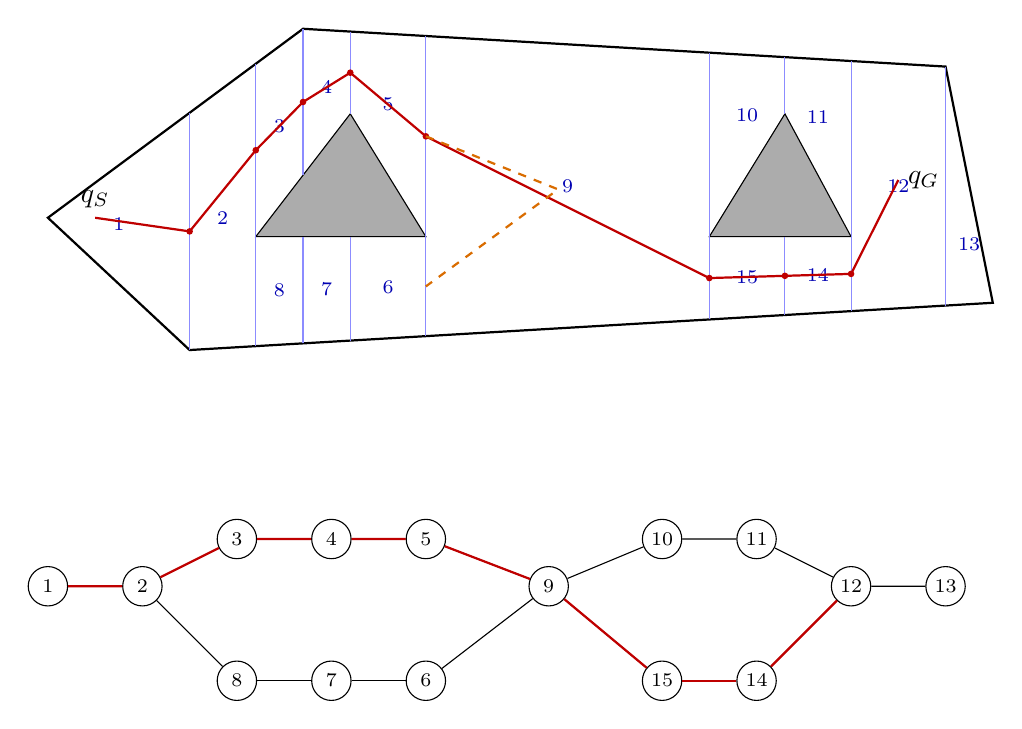
\begin{tikzpicture}[scale=1.2]
\draw[thick] (0.0000,1.4000)--(2.7000,3.4000)--(9.5000,3.0000)--(10.0000,0.5000)--(1.5000,0.0000)--cycle;
\filldraw[fill=gray!65] (2.2000,1.2000)--(3.2000,2.5000)--(4.0000,1.2000)--cycle;
\filldraw[fill=gray!65] (7.0000,1.2000)--(7.8000,2.5000)--(8.5000,1.2000)--cycle;
\draw[thin,blue!45] (1.5000,0.0000)--(1.5000,2.5111);
\draw[thin,blue!45] (2.2000,0.0412)--(2.2000,1.2000);
\draw[thin,blue!45] (2.2000,1.2000)--(2.2000,3.0296);
\draw[thin,blue!45] (2.7000,0.0706)--(2.7000,1.2000);
\draw[thin,blue!45] (2.7000,1.8500)--(2.7000,3.4000);
\draw[thin,blue!45] (3.2000,0.1000)--(3.2000,1.2000);
\draw[thin,blue!45] (3.2000,2.5000)--(3.2000,3.3706);
\draw[thin,blue!45] (4.0000,0.1471)--(4.0000,1.2000);
\draw[thin,blue!45] (4.0000,1.2000)--(4.0000,3.3235);
\draw[thin,blue!45] (7.0000,0.3235)--(7.0000,1.2000);
\draw[thin,blue!45] (7.0000,1.2000)--(7.0000,3.1471);
\draw[thin,blue!45] (7.8000,0.3706)--(7.8000,1.2000);
\draw[thin,blue!45] (7.8000,2.5000)--(7.8000,3.1000);
\draw[thin,blue!45] (8.5000,0.4118)--(8.5000,1.2000);
\draw[thin,blue!45] (8.5000,1.2000)--(8.5000,3.0588);
\draw[thin,blue!45] (9.5000,0.4706)--(9.5000,3.0000);
\node[blue!70!black,font=\scriptsize] at (0.7500,1.3278) {1};
\node[blue!70!black,font=\scriptsize] at (1.8500,1.3955) {2};
\node[blue!70!black,font=\scriptsize] at (2.4500,0.6279) {8};
\node[blue!70!black,font=\scriptsize] at (2.4500,2.3699) {3};
\node[blue!70!black,font=\scriptsize] at (2.9500,0.6426) {7};
\node[blue!70!black,font=\scriptsize] at (2.9500,2.7801) {4};
\node[blue!70!black,font=\scriptsize] at (3.6000,0.6618) {6};
\node[blue!70!black,font=\scriptsize] at (3.6000,2.5985) {5};
\node[blue!70!black,font=\scriptsize] at (5.5000,1.7353) {9};
\node[blue!70!black,font=\scriptsize] at (7.4000,0.7735) {15};
\node[blue!70!black,font=\scriptsize] at (7.4000,2.4868) {10};
\node[blue!70!black,font=\scriptsize] at (8.1500,0.7956) {14};
\node[blue!70!black,font=\scriptsize] at (8.1500,2.4647) {11};
\node[blue!70!black,font=\scriptsize] at (9.0000,1.7353) {12};
\node[blue!70!black,font=\scriptsize] at (9.7500,1.1176) {13};
\draw[red!75!black,thick] (0.5000,1.4000)--(1.5000,1.2556)--(2.2000,2.1148)--(2.7000,2.6250)--(3.2000,2.9353)--(4.0000,2.2618)--(7.0000,0.7618)--(7.8000,0.7853)--(8.5000,0.8059)--(9.0000,1.8000);
\fill[red!75!black] (1.5000,1.2556) circle(.035);
\fill[red!75!black] (2.2000,2.1148) circle(.035);
\fill[red!75!black] (2.7000,2.6250) circle(.035);
\fill[red!75!black] (3.2000,2.9353) circle(.035);
\fill[red!75!black] (4.0000,2.2618) circle(.035);
\fill[red!75!black] (7.0000,0.7618) circle(.035);
\fill[red!75!black] (7.8000,0.7853) circle(.035);
\fill[red!75!black] (8.5000,0.8059) circle(.035);
\node[above] at (0.5000,1.4000) {$q_S$};
\node[right] at (9.0000,1.8000) {$q_G$};
\draw[orange!85!black,thick,dashed] (4.0000,2.2618)--(5.4,1.7)--(4.0000,0.6735);
\begin{scope}[yshift=-3.5cm,n/.style={circle,draw,fill=white,minimum size=5mm,inner sep=1pt,font=\scriptsize}]
\node[n] (n1) at (0.0000,1.0000) {1};
\node[n] (n2) at (1.0000,1.0000) {2};
\node[n] (n3) at (2.0000,1.5000) {3};
\node[n] (n4) at (3.0000,1.5000) {4};
\node[n] (n5) at (4.0000,1.5000) {5};
\node[n] (n9) at (5.3000,1.0000) {9};
\node[n] (n10) at (6.5000,1.5000) {10};
\node[n] (n11) at (7.5000,1.5000) {11};
\node[n] (n12) at (8.5000,1.0000) {12};
\node[n] (n13) at (9.5000,1.0000) {13};
\node[n] (n8) at (2.0000,0.0000) {8};
\node[n] (n7) at (3.0000,0.0000) {7};
\node[n] (n6) at (4.0000,0.0000) {6};
\node[n] (n15) at (6.5000,0.0000) {15};
\node[n] (n14) at (7.5000,0.0000) {14};
\draw (n1)--(n2);
\draw (n2)--(n3);
\draw (n2)--(n8);
\draw (n3)--(n4);
\draw (n4)--(n5);
\draw (n8)--(n7);
\draw (n7)--(n6);
\draw (n5)--(n9);
\draw (n6)--(n9);
\draw (n9)--(n10);
\draw (n10)--(n11);
\draw (n11)--(n12);
\draw (n9)--(n15);
\draw (n15)--(n14);
\draw (n14)--(n12);
\draw (n12)--(n13);
\draw[red!75!black,thick] (n1)--(n2);
\draw[red!75!black,thick] (n2)--(n3);
\draw[red!75!black,thick] (n3)--(n4);
\draw[red!75!black,thick] (n4)--(n5);
\draw[red!75!black,thick] (n5)--(n9);
\draw[red!75!black,thick] (n9)--(n15);
\draw[red!75!black,thick] (n15)--(n14);
\draw[red!75!black,thick] (n14)--(n12);
\end{scope}
\end{tikzpicture}
